\section{Gestione dei Requisiti}
\subsection{Requisiti progettuali}
	\subsubsection{Diagramma}
		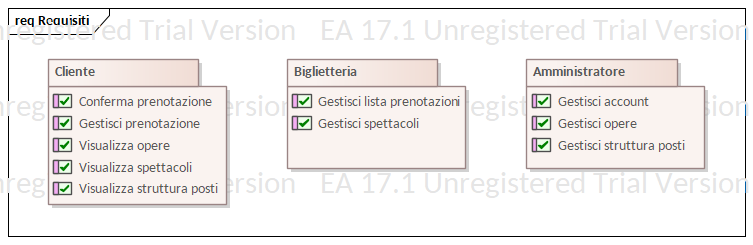
\includegraphics{imgs/requisiti/requisiti}
	
	\subsubsection{Requisiti Funzionali}
		\newcounter{rf}
		
		\textbf{Area Cliente} \\
		\textbf{RF\mycount{rf}: Visualizza opere} \\ Il sistema dovrà mostrare al cliente le anagrafiche delle opere e l'archivio delle relative regie. \\ \\
		\textbf{RF\mycount{rf}: Visualizza spettacoli} \\ Il sistema dovrà mostrare al cliente la lista degli spettacoli e dei relativi eventi disponibili all'acquisto. \\ \\
		\textbf{RF\mycount{rf}: Visualizza struttura posti} \\ Il sistema dovrà consentire al cliente di visualizzare la struttura posti del teatro durante la composizione della prenotazione. \\ \\
		\textbf{RF\mycount{rf}: Gestisci prenotazione} \\ Il sistema dovrà consentire al cliente di creare una prenotazione e modificarne i posti o eliminarla completamente prima di averla confermata. \\ \\
		\textbf{RF\mycount{rf}: Conferma prenotazione} \\ Il sistema dovrà consentire al cliente di confermare la prenotazione, e produrre la ricevuta contenente l'identificativo della prenotazione per il pagamento alla cassa. \\ \\
		
		\noindent \textbf{Area Biglietteria} \\
		\textbf{RF\mycount{rf}: Gestisci spettacoli} \\ Il sistema dovrà consentire alla biglietteria di creare, modificare e rimuovere gli spettacoli in programma e i relativie eventi. \\ \\
		\textbf{RF\mycount{rf}: Gestisci lista prenotazioni} \\ Il sistema dovrà consentire alla biglietteria di visualizzare e modificare tutte le prenotazioni effettuate nel teatro e di contrassegnare le prenotazioni che sono state pagate in cassa. \\ \\
		
		\noindent \textbf{Area Amministratore} \\
		\textbf{RF\mycount{rf}: Gestisci opere} \\ Il sistema dovrà consentire all'amministratore di creare, modificare e rimuovere le anagrafiche delle opere e l'archivio delle relative regie. \\ \\
		\textbf{RF\mycount{rf}: Gestisci struttura posti} \\ Il sistema dovrà consentire all'amministratore di modificare la struttura posti del teatro. \\
		
	\subsubsection{Requisiti Non Funzionali}
		\newcounter{rnf}
		
		\textbf{RNF\mycount{rnf}: Python3} \\ Il sistema dovrà essere implementato in linguaggio Python3. \\
\newpage

	\subsection{Casi d'uso}
		\subsubsection{Attori}
			\textbf{Diagramma} \\ \\ 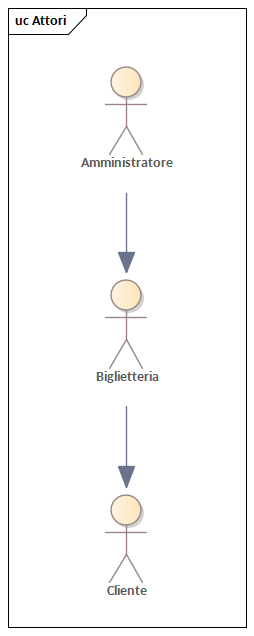
\includegraphics{imgs/use_case/attori}
			\newpage
	
		\subsubsection{Cliente}
			\textbf{Diagramma} \\ \\ 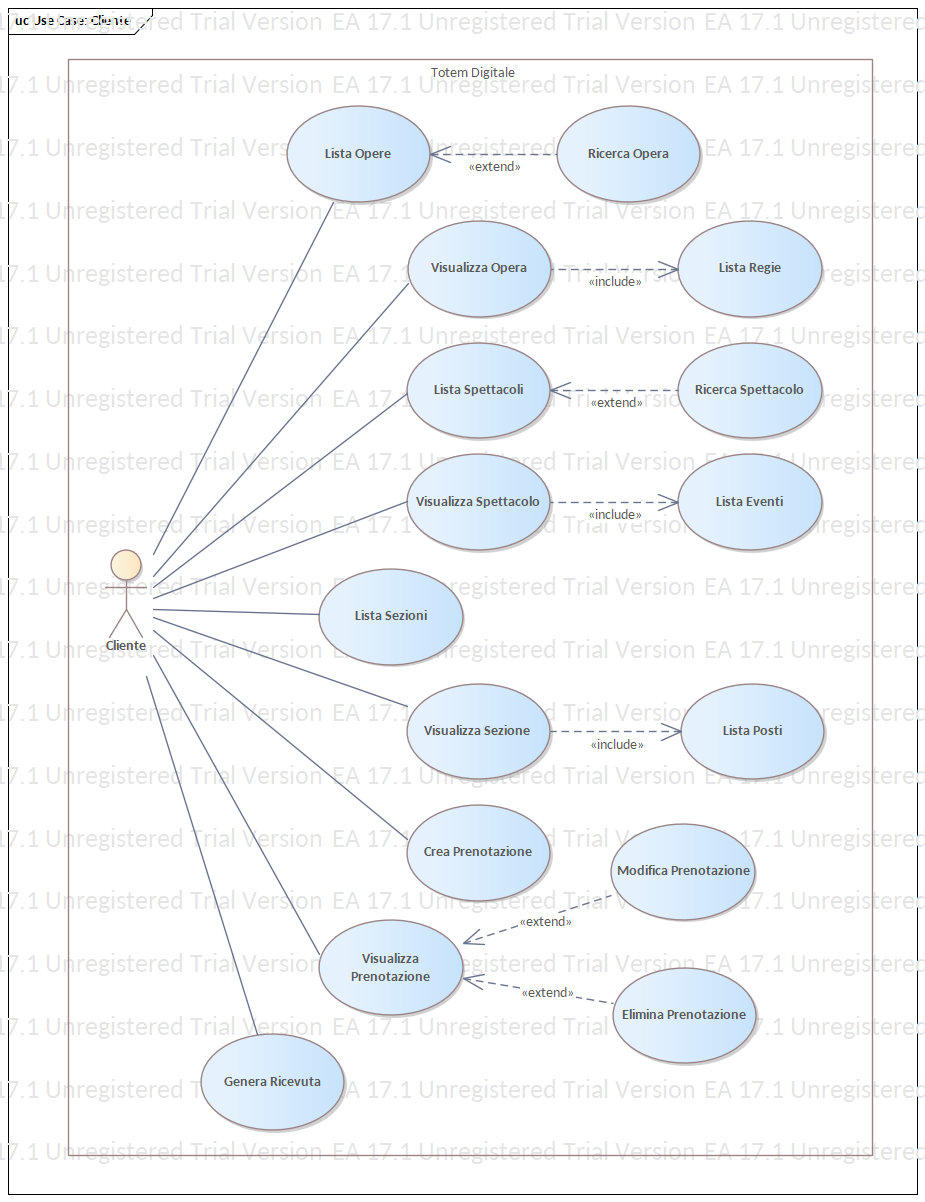
\includegraphics[scale=0.8]{imgs/use_case/cliente}
			\newpage
		
			\textbf{Descrizioni}
			% UC: Lista Opere
\begin{table}[H]
    \begin{tabular}{|p{\linewidth}|}
        \hline
        \cellcolor{gray!100}
        \color{white}
        \centerline{\textbf{Caso d'uso:} Lista Opere} \\
        \hline
        \textbf{ID:} 1 \\
        \hline
        \cellcolor{gray!20}
        \textbf{Breve descrizione:} \\
        \cellcolor{gray!20}
        L'utente ottiene la lista di opere memorizzate nel sistema. \\
        \hline
        \textbf{Attori primari:} \\
        \begin{minipage}{\linewidth}
            Cliente \\
            Biglietteria \\
            Amministratore
        \end{minipage}
        \vspace{0pt} \\  % Utilizzo \vspace{} per regolare lo spazio tra le sezioni delle tabelle.
        \hline
        \textbf{Attori secondari:} \\
        Nessuno. \\
        \hline
        \cellcolor{gray!20}
        \textbf{Precondizioni:} \\
        \cellcolor{gray!20}
        \begin{minipage}{\linewidth}
            \begin{enumerate}
                \item L'utente è posizionato nella sezione informazioni.
            \end{enumerate}
        \end{minipage} \\
        \hline
        \textbf{Sequenza degli eventi principale:}
        \begin{enumerate}
            \item Il caso d'uso inizia quando l'utente entra nella sezione informazioni.
            \item \textbf{If} nel sistema è memorizzata almeno un'opera
            \begin{enumerate}
                \item \textbf{For} ogni opera nel sistema
                \begin{enumerate}
                    \item[] \textbf{punto di estensione:} filtro ricerca
                    \item Vengono visualizzate le informazioni essenziali dell'opera.
                \end{enumerate}
            \end{enumerate}
            \item \textbf{Else}
            \begin{enumerate}
                \item Il sistema informa l'utente che non vi sono opere memorizzate.
            \end{enumerate}
        \end{enumerate} \\
        \hline
        \cellcolor{gray!20}
        \textbf{Postcondizioni:} \\
        \cellcolor{gray!20}
        \begin{minipage}{\linewidth}
            \begin{enumerate}
                \item Viene visualizzata a schermo la lista delle opere memorizzate.
            \end{enumerate}
        \end{minipage} \\
        \hline
        \textbf{Sequenza degli eventi alternativa:} \\
        Nessuna. \\
        \hline
    \end{tabular}
\end{table}

% UC EXT: Ricerca Opera
\begin{table}[H]
    \begin{tabular}{|p{\linewidth}|}
        \hline
        \cellcolor{gray!100}
        \color{white}
        \centerline{\textbf{Caso d'uso di estensione:} Ricerca Opera} \\
        \hline
        \textbf{ID:} 2 \\
        \hline
        \cellcolor{gray!20}
        \textbf{Breve descrizione:} \\
        \cellcolor{gray!20}
        \textbf{Segmento 1:} L'utente filtra la lista di opere tramite parola chiave ricercata nel nome. \\
        \hline
        \textbf{Attori primari:} \\
        \begin{minipage}{\linewidth}
            Cliente \\
            Biglietteria \\
            Amministratore
        \end{minipage}
        \vspace{0pt} \\  % Utilizzo \vspace{} per regolare lo spazio tra le sezioni delle tabelle.
        \hline
        \textbf{Attori secondari:} \\
        Nessuno. \\
        \hline
        \cellcolor{gray!20}
        \textbf{Precondizioni del segmento 1:} \\
        \cellcolor{gray!20}
        \begin{minipage}{\linewidth}
            \begin{enumerate}
                \item L'utente ha inserito una chiave di ricerca.
                \item L'utente ha premuto il pulsante di ricerca.
            \end{enumerate}
        \end{minipage} \\
        \hline
        \textbf{Sequenza degli eventi principale del segmento 1:}
        \begin{enumerate}
            \item Le opere che non contengono la parola chiave vengono eliminate dalla lista risultante.
        \end{enumerate} \\
        \hline
        \cellcolor{gray!20}
        \textbf{Postcondizioni del segmento 1:} \\
        \cellcolor{gray!20}
        \begin{minipage}{\linewidth}
            \begin{enumerate}
                \item La lista risultante è filtrata.
            \end{enumerate}
        \end{minipage} \\
        \hline
    \end{tabular}
\end{table}

% UC: Visualizza Opera
\begin{table}[H]
    \begin{tabular}{|p{\linewidth}|}
        \hline
        \cellcolor{gray!100}
        \color{white}
        \centerline{\textbf{Caso d'uso:} Visualizza Opera} \\
        \hline
        \textbf{ID:} 3 \\
        \hline
        \cellcolor{gray!20}
        \textbf{Breve descrizione:} \\
        \cellcolor{gray!20}
        L'utente ottiene le informazioni anagrafiche riguardo una singola opera. \\
        \hline
        \textbf{Attori primari:} \\
        \begin{minipage}{\linewidth}
            Cliente \\
            Biglietteria \\
            Amministratore
        \end{minipage}
        \vspace{0pt} \\ % Utilizzo \vspace{} per regolare lo spazio tra le sezioni delle tabelle.
        \hline
        \textbf{Attori secondari:} \\
        Nessuno. \\
        \hline
        \cellcolor{gray!20}
        \textbf{Precondizioni:} \\
        \cellcolor{gray!20}
        \begin{minipage}{\linewidth}
            \begin{enumerate}
                \item L'utente è posizionato nella sezione informazioni.
            \end{enumerate}
        \end{minipage} \\
        \hline
        \textbf{Sequenza degli eventi principale:}
        \begin{enumerate}
            \item Il caso d'uso inizia quando l'utente richiede le informazioni di un'opera.
            \item Il sistema cerca le informazioni anagrafiche nella memoria.
            \item Il sistema mostra le informazioni a schermo.
            \item \textbf{include}(Lista Regie)
            \item[] \textbf{punto di estensione:} modifica
        \end{enumerate} \\
        \hline
        \cellcolor{gray!20}
        \textbf{Postcondizioni:} \\
        \cellcolor{gray!20}
        \begin{minipage}{\linewidth}
            \begin{enumerate}
                \item Sono visualizzate a schermo le informazioni anagrafiche dell'opera.
            \end{enumerate}
        \end{minipage} \\
        \hline
        \textbf{Sequenza degli eventi alternativa:} \\
        Nessuna. \\
        \hline
    \end{tabular}
\end{table}

% UC: Lista Regie
\begin{table}[H]
    \begin{tabular}{|p{\linewidth}|}
        \hline
        \cellcolor{gray!100}
        \color{white}
        \centerline{\textbf{Caso d'uso:} Lista Regie} \\
        \hline
        \textbf{ID:} 4 \\
        \hline
        \cellcolor{gray!20}
        \textbf{Breve descrizione:} \\
        \cellcolor{gray!20}
        L'utente ottiene la lista di regie relative all'opera che sta visualizzando. \\
        \hline
        \textbf{Attori primari:} \\
        \begin{minipage}{\linewidth}
            Cliente \\
            Biglietteria \\
            Amministratore
        \end{minipage}
        \vspace{0pt} \\ % Utilizzo \vspace{} per regolare lo spazio tra le sezioni delle tabelle.
        \hline
        \textbf{Attori secondari:} \\
        Nessuno. \\
        \hline
        \cellcolor{gray!20}
        \textbf{Precondizioni:} \\
        \cellcolor{gray!20}
        \begin{minipage}{\linewidth}
            \begin{enumerate}
                \item L'utente sta visualizzando una singola opera.
            \end{enumerate}
        \end{minipage} \\
        \hline
        \textbf{Sequenza degli eventi principale:}
        \begin{enumerate}
            \item Il caso d'uso inizia quando l'utente visualizza una singola opera.
            \item \textbf{If} per l'opera è memorizzata almeno una regia
            \begin{enumerate}
                \item \textbf{For} ogni regia dell'opera
                \begin{enumerate}
                    \item Il sistema mostra le informazioni della regia a schermo.
                \end{enumerate}
            \end{enumerate}
            \item \textbf{Else}
            \begin{enumerate}
                \item Il sistema informa l'utente che non vi sono regie memorizzate.
            \end{enumerate}
        \end{enumerate} \\
        \hline
        \cellcolor{gray!20}
        \textbf{Postcondizioni:} \\
        \cellcolor{gray!20}
        \begin{minipage}{\linewidth}
            \begin{enumerate}
                \item E' visualizzata a schermo la lista delle regie associate all'opera.
            \end{enumerate}
        \end{minipage} \\
        \hline
        \textbf{Sequenza degli eventi alternativa:} \\
        Nessuna. \\
        \hline
    \end{tabular}
\end{table}

% UC: Lista Spettacoli
\begin{table}[H]
    \begin{tabular}{|p{\linewidth}|}
        \hline
        \cellcolor{gray!100}
        \color{white}
        \centerline{\textbf{Caso d'uso:} Lista Spettacoli} \\
        \hline
        \textbf{ID:} 5 \\
        \hline
        \cellcolor{gray!20}
        \textbf{Breve descrizione:} \\
        \cellcolor{gray!20}
        L'utente visualizzare l'elenco degli spettacoli disponibili presso il teatro. \\
        \hline
        \textbf{Attori primari:} \\
        \begin{minipage}{\linewidth}
            Cliente \\
            Biglietteria \\
            Amministratore \\
        \end{minipage}
        \vspace{-10pt} \\ 
        \hline
        \textbf{Attori secondari:} \\
        Nessuno. \\
        \hline
        \cellcolor{gray!20}
        \textbf{Precondizioni:} \\
        \cellcolor{gray!20}
        \begin{minipage}{\linewidth}
            \begin{enumerate}
                \item L'utente è posizionato nella sezione informazione.
            \end{enumerate}
        \end{minipage} \\
        \hline
        \textbf{Sequenza degli eventi principale:}
        \begin{enumerate}
            \item Il caso d'uso inizia quando l'utente richiede di visualizzare la lista completa degli spettacoli.
            \item \textbf{If} c'è almeno uno spettacolo memorizzato nel Sistema
            \begin{enumerate}
                \item \textbf{For} ogni spettacolo nel Sistema
                \begin{enumerate}
                    \item Il sistema mostra un'anteprima dello spettacolo con informazioni basiche (es. titolo, data, genere). % Disponibilità?
                \end{enumerate}
                \item[] \textbf{punto di estensione:} filtrareElenco
            \end{enumerate}
            \item \textbf{Else}
            \begin{enumerate}
                \item Il Sistema informa l'utente che non vi sono spettacoli memorizzati.
            \end{enumerate}
        \end{enumerate} \\
        \hline
        \cellcolor{gray!20}
        \textbf{Postcondizioni:} \\
        \cellcolor{gray!20}
        \begin{minipage}{\linewidth}
            \begin{enumerate}
                \item Viene visualizzata a schermo la lista degli spettacoli memorizzati.
            \end{enumerate}
        \end{minipage} \\
        \hline
        \textbf{Sequenza degli eventi alternativa:} \\
        Nessuna. \\
        \hline
    \end{tabular}
\end{table}

% UC EXT: Ricerca Spettacolo
\begin{table}[H]
    \begin{tabular}{|p{\linewidth}|}
        \hline
        \cellcolor{gray!100}
        \color{white}
        \centerline{\textbf{Caso d'uso di estensione:} Ricerca Spettacolo} \\
        \hline
        \textbf{ID:} 6 \\
        \hline
        \cellcolor{gray!20}
        \textbf{Breve descrizione:} \\
        \cellcolor{gray!20}
        \textbf{Segmento 1:} L'utente filtra la lista di spettacoli applicando eventuali filtri (es. titolo, data, genere). \\
        \hline
        \textbf{Attori primari:} \\
        \begin{minipage}{\linewidth}
            Cliente \\
            Biglietteria \\
            Amministratore \\
        \end{minipage}
        \vspace{-10pt} \\ 
        \hline
        \textbf{Attori secondari:} \\
        Nessuno. \\
        \hline
        \cellcolor{gray!20}
        \textbf{Precondizioni del segmento 1:} \\
        \cellcolor{gray!20}
        \begin{minipage}{\linewidth}
            \begin{enumerate}
                \item L'utente ha inserito i criteri di ricerca.
                \item L'utente ha premuto il pulsante di ricerca.
            \end{enumerate}
        \end{minipage} \\
        \hline
        \textbf{Sequenza degli eventi principale del segmento 1:}
        \begin{enumerate}
            \item Il Sistema ricerca, nell'elenco di spettacoli, degli spettacoli coincidenti.
            \item \textbf{If} il Sistema trova almeno uno spettacolo coincidente
            \begin{enumerate}
                \item \textbf{For} ogni spettacolo coincidente
                \begin{enumerate}
                    \item Il sistema mostra un'anteprima dello spettacolo con informazioni basiche.
                \end{enumerate}
            \end{enumerate}
            \item \textbf{Else}
            \begin{enumerate}
                \item Il Sistema informa l'utente che non vi sono spettacoli coincidenti.
            \end{enumerate}
        \end{enumerate} \\
        \hline
        \cellcolor{gray!20}
        \textbf{Postcondizioni del segmento 1:} \\
        \cellcolor{gray!20}
        \begin{minipage}{\linewidth}
            \begin{enumerate}
                \item L'utente visualizza l'elenco filtrato.
            \end{enumerate}
        \end{minipage} \\
        \hline
    \end{tabular}
\end{table}

% UC: Visualizza Spettacolo
\begin{table}[H]
    \begin{tabular}{|p{\linewidth}|}
        \hline
        \cellcolor{gray!100}
        \color{white}
        \centerline{\textbf{Caso d'uso:} Visualizza Spettacolo} \\
        \hline
        \textbf{ID:} 7 \\
        \hline
        \cellcolor{gray!20}
        \textbf{Breve descrizione:} \\
        \cellcolor{gray!20}
        L'utente visualizza i dettagli di uno spettacolo selezionato dalla lista. \\
        \hline
        \textbf{Attori primari:} \\
        \begin{minipage}{\linewidth}
            Cliente \\
            Biglietteria \\
            Amministratore \\
        \end{minipage}
        \vspace{-10pt} \\ 
        \hline
        \textbf{Attori secondari:} \\
        Nessuno. \\
        \hline
        \cellcolor{gray!20}
        \textbf{Precondizioni:} \\
        \cellcolor{gray!20}
        \begin{minipage}{\linewidth}
            \begin{enumerate}
                \item L'utente visualizza la lista degli spettacoli.
                \item L'utente ha selezionato uno spettacolo della lista.
            \end{enumerate}
        \end{minipage} \\
        \hline
        \textbf{Sequenza degli eventi principale:}
        \begin{enumerate}
            \item Il Sistema mostra tutti i dettagli dello spettacolo: titolo, descrizione, durata, ecc.
            \item \textbf{include}(Lista Eventi)
            \item \textbf{If} l'utente è autenticato come Amministratore
            \begin{enumerate}
                \item[] \textbf{punto di estensione:} modificaSpettacolo
            \end{enumerate}
        \end{enumerate} \\
        \hline
        \cellcolor{gray!20}
        \textbf{Postcondizioni:} \\
        \cellcolor{gray!20}
        \begin{minipage}{\linewidth}
            \begin{enumerate}
                \item Sono visualizzate a schermo le informazioni anagrafiche dello spettacolo.
            \end{enumerate}
        \end{minipage} \\
        \hline
        \textbf{Sequenza degli eventi alternativa:} \\
        Nessuna. \\
        \hline
    \end{tabular}
\end{table}

% UC: Lista Eventi
\begin{table}[H]
    \begin{tabular}{|p{\linewidth}|}
        \hline
        \cellcolor{gray!100}
        \color{white}
        \centerline{\textbf{Caso d'uso:} Lista Eventi} \\
        \hline
        \textbf{ID:} 8 \\
        \hline
        \cellcolor{gray!20}
        \textbf{Breve descrizione:} \\
        \cellcolor{gray!20}
        L'utente visualizza l'elenco di tutti gli eventi programmati per uno spettacolo. \\
        \hline
        \textbf{Attori primari:} \\
        \begin{minipage}{\linewidth}
            Cliente \\
            Biglietteria \\
            Amministratore \\
        \end{minipage}
        \vspace{-10pt} \\ 
        \hline
        \textbf{Attori secondari:} \\
        Nessuno. \\
        \hline
        \cellcolor{gray!20}
        \textbf{Precondizioni:} \\
        \cellcolor{gray!20}
        \begin{minipage}{\linewidth}
            \begin{enumerate}
                \item L'utente visualizza i dettagli di uno spettacolo.
            \end{enumerate}
        \end{minipage} \\
        \hline
        \textbf{Sequenza degli eventi principale:}
        \begin{enumerate}
            \item Il caso d'uso inizia dopo che l'utente visualizza i dettagli di uno spettacolo.
            \item \textbf{For} ogni eventi vincolato allo spettacolo
            \begin{enumerate}
                \item Il Sistema mostra informazioni rilevanti dell'evento (es. data, ora, sala).
            \end{enumerate}
        \end{enumerate} \\
        \hline
        \cellcolor{gray!20}
        \textbf{Postcondizioni:} \\
        \cellcolor{gray!20}
        \begin{minipage}{\linewidth}
            \begin{enumerate}
                \item E' visualizzata a schermo la lista degli eventi associati allo spettacolo.
            \end{enumerate}
        \end{minipage} \\
        \hline
        \textbf{Sequenza degli eventi alternativa:} \\
        Nessuna. \\
        \hline
    \end{tabular}
\end{table}

% UC: Lista Sezioni
\begin{table}[H]
    \begin{tabular}{|p{\linewidth}|}
        \hline
        \cellcolor{gray!100}
        \color{white}
        \centerline{\textbf{Caso d'uso:} Lista Sezioni} \\ 
        \hline
        \textbf{ID:} 9 \\
        \hline
        \cellcolor{gray!20}
        \textbf{Breve descrizione:} \\
        \cellcolor{gray!20}
        Messa a schermo delle sezioni. \\
        \hline
        \textbf{Attori primari:} \\
        \begin{minipage}{\linewidth}
            Cliente \\
            Biglietteria \\
            Amministratore 
        \end{minipage}
        \vspace{0pt} \\  % Utilizzo \vspace{} per regolare lo spazio tra le sezioni delle tabelle.
        \hline
        \textbf{Attori secondari:} \\
        Nessuno. \\
        \hline
        \cellcolor{gray!20}
        \textbf{Precondizioni:} \\
        \cellcolor{gray!20}
        \begin{minipage}{\linewidth}
            \begin{enumerate}
            	\item L'utente si trova nella categoria "Sezioni \& Posti"
                \item L'utente sta visualizzando l'elenco delle sezioni.
            \end{enumerate}
        \end{minipage} 
        \vspace{0pt} \\
        \hline
        \textbf{Sequenza degli eventi principale:}
        \begin{enumerate}
            \item Il caso d'uso inizia quando l'utente seleziona \textit{Sezioni}.
            \item \textbf{include}(Visualizza Sezione)
            \item \textbf{If} esistono sezioni
            \begin{enumerate}
                \item Il Sistema mostra all'utente tutte le Sezioni presenti una dopo l'altra.
            \end{enumerate}
            \item \textbf{Else}
            \begin{enumerate}
                \item Il Sistema comunica che la lista delle Sezioni è vuota.
                \item Il Sistema mostra un elenco vuoto.
            \end{enumerate}				
        \end{enumerate} \\
        \hline
        \cellcolor{gray!20}
        \textbf{Postcondizioni:} \\
        \cellcolor{gray!20}
        \begin{minipage}{\linewidth}
            \begin{enumerate}
                \item Il Sistema ha elencato le Sezioni presenti.
            \end{enumerate}
        \end{minipage} \\
        \hline
        \textbf{Sequenza degli eventi alternativa:} \\
        Nessuna. \\
        \hline
    \end{tabular}
\end{table}

% UC: Visualizza Sezione
\begin{table}[H]
    \begin{tabular}{|p{\linewidth}|}
        \hline
        \cellcolor{gray!100}
        \color{white}
        \centerline{\textbf{Caso d'uso:} Visualizza Sezione} \\
        \hline
        \textbf{ID:} 10 \\
        \hline
        \cellcolor{gray!20}
        \textbf{Breve descrizione:} \\
        \cellcolor{gray!20}
        Visualizzazione con dettagli di una sezione. \\
        \hline
        \textbf{Attori primari:} \\
        \begin{minipage}{\linewidth}
            Amministratore \\
            Biglietteria \\
            Cliente
        \end{minipage}
        \vspace{0pt} \\ 
        \hline
        \textbf{Attori secondari:} \\
        Nessuno. \\
        \hline
        \cellcolor{gray!20}
        \textbf{Precondizioni:} \\
        \cellcolor{gray!20}
        \begin{minipage}{\linewidth}
            \begin{enumerate}
                \item L'utente sta ha richiesto la lista delle sezioni.
            \end{enumerate}
        \end{minipage} \\
        \hline
        \textbf{Sequenza degli eventi principale:}
        \begin{enumerate}
            \item Il caso d'uso inizia quando l'utente visualizza una Sezione.
            \item \textbf{include}(Lista Posti)
            \item Il Sistema mostra all'utente i dati della Sezione.
            \item Il Sistema mostra il pulsante \textit{Lista Posti}.
            \item \textbf{If} l'utente è autenticato come Amministratore
            \begin{enumerate}
                \item Il Sistema mostra, accanto al primo pulsante, altre due opzioni: \textit{Modifica Sezione} e \textit{Elimina Sezione}.
                \item[] \textbf{punto di estensione}: modificaSezione, eliminaSezione
            \end{enumerate}
        \end{enumerate} \\
        \hline
        \cellcolor{gray!20}
        \textbf{Postcondizioni:} \\
        \cellcolor{gray!20}
        \begin{minipage}{\linewidth}
            \begin{enumerate}
                \item Il Sistema ha mostrato i dati della Sezione.
                \item Il Sistema dà l'opzione di visualizzare i posti relativi alla Sezione.
                \item Se l'utente è Amministratore, il Sistema permette di modificare o eliminare la sezione.
            \end{enumerate}
        \end{minipage} \\
        \hline
        \textbf{Sequenza degli eventi alternativa:} \\
        Nessuna. \\
        \hline
    \end{tabular}
\end{table}

% UC: Lista Posti
\begin{table}[H]
    \begin{tabular}{|p{\linewidth}|}
        \hline
        \cellcolor{gray!100}
        \color{white}
        \centerline{\textbf{Caso d'uso:} Lista Posti} \\
        \hline
        \textbf{ID:} 11 \\
        \hline
        \cellcolor{gray!20}
        \textbf{Breve descrizione:} \\
        \cellcolor{gray!20}
        Messa a schermo dei posti. \\
        \hline
        \textbf{Attori primari:} \\
        \begin{minipage}{\linewidth}
            Amministratore \\
            Biglietteria \\ 
            Cliente
        \end{minipage}
        \vspace{0pt} \\ 
        \hline
        \textbf{Attori secondari:} \\
        Nessuno. \\
        \hline
        \cellcolor{gray!20}
        \textbf{Precondizioni:} \\
        \cellcolor{gray!20}
        \begin{minipage}{\linewidth}
            \begin{enumerate}
                \item È stato caricato in memoria un database valido. 
            \end{enumerate}
        \end{minipage} 
        \vspace{-10pt} \\
        \hline
        \textbf{Sequenza degli eventi principale:}
        \begin{enumerate}
            \item Il caso d'uso inizia quando l'utente seleziona \textit{Posti} all'interno di una Sezione.
            \item \textbf{If} la Sezione contiene Posti
            \begin{enumerate}
                \item Il Sistema mostra all'utente tutti i Posti presenti della Sezione sotto forma di elenco.
            \end{enumerate}
            \item \textbf{Else}
            \begin{enumerate}
                \item Il Sistema comunica che la lista dei Posti della Sezione è vuota.
                \item Il Sistema mostra un elenco vuoto.
            \end{enumerate}				
        \end{enumerate} \\
        \hline
        \cellcolor{gray!20}
        \textbf{Postcondizioni:} \\
        \cellcolor{gray!20}
        \begin{minipage}{\linewidth}
            \begin{enumerate}
                \item Il Sistema ha elencato i Posti della Sezione selezionata.
            \end{enumerate}
        \end{minipage} \\
        \hline
        \textbf{Sequenza degli eventi alternativa:} \\
        Nessuna. \\
        \hline
    \end{tabular}
\end{table}

% UC: Crea Prenotazione
\begin{table}[H]
    \begin{tabular}{|p{\linewidth}|}
        \hline
        \cellcolor{gray!100}
        \color{white}
        \centerline{\textbf{Caso d'uso:} Crea Prenotazione} \\
        \hline
        \textbf{ID:} 12 \\
        \hline
        \cellcolor{gray!20}
        \textbf{Breve descrizione:} \\
        \cellcolor{gray!20}
        L'utente prenota posti di un evento svolto nel teatro. \\
        \hline
        \textbf{Attori primari:} \\
        \begin{minipage}{\linewidth}
            Cliente \\
            Biglietteria \\
            Amministratore
        \end{minipage}
        \vspace{0pt} \\
        \hline
        \textbf{Attori secondari:} \\                        
        Nessuno. \\
        \hline
        \cellcolor{gray!20}
        \textbf{Precondizioni:} \\
        \cellcolor{gray!20}
        \begin{minipage}{\linewidth}
            \begin{enumerate}
                \item L'utente visualizza l'elenco degli eventi.
            \end{enumerate}
        \end{minipage} \\
        \hline
        \textbf{Sequenza degli eventi principale:}
        \begin{enumerate}
            \item Il caso d'uso inizia quando l'utente preme il pulsante di creazione.
            \item Il Sistema, tramite un'interfaccia, permette di inserire i dati relativi alla prenotazione.
            \item L'utente inserisce i dati relativi alla prenotazione.
            \item L'utente salva i dati.
            \item Il Sistema verifica i dati e li salva in memoria.
        \end{enumerate} \\
        \hline
        \cellcolor{gray!20}
        \textbf{Postcondizioni:} \\
        \cellcolor{gray!20}
        \begin{minipage}{\linewidth}
            \begin{enumerate}
                \item L'utente crea una prenotazione.
            \end{enumerate}
        \end{minipage}
        \vspace{-10pt} \\
        \hline
        \textbf{Sequenza degli eventi alternativa:} \\
        Nessuna. \\
        \hline
    \end{tabular}
\end{table}

% UC: Visualizza Prenotazione
\begin{table}[H]
    \begin{tabular}{|p{\linewidth}|}
        \hline
        \cellcolor{gray!100}
        \color{white}
        \centerline{\textbf{Caso d'uso:} Visualizza Prenotazione} \\
        \hline
        \textbf{ID:} 13 \\
        \hline
        \cellcolor{gray!20}
        \textbf{Breve descrizione:} \\
        \cellcolor{gray!20}
        L'utente ottiene l'informazione anagrafica riguardo una singola prenotazione. \\
        \hline
        \textbf{Attori primari:} \\
        \begin{minipage}{\linewidth}
            Cliente \\
            Biglietteria \\
            Amministratore
        \end{minipage}
        \vspace{0pt} \\
        \hline
        \textbf{Attori secondari:} \\
        Nessuno. \\
        \hline
        \cellcolor{gray!20}
        \textbf{Precondizioni:} \\
        \cellcolor{gray!20}
        \begin{minipage}{\linewidth}
            \begin{enumerate}
                \item L'utente visualizza la lista delle prenotazioni.
                \item L'elenco delle prenotazioni, sia esso filtrato o meno, non è vuoto.
            \end{enumerate}
        \end{minipage}
        \vspace{-5pt} \\
        \hline
        \textbf{Sequenza degli eventi principale:}
        \begin{enumerate}
            \item Il caso d'uso inizia quando l'utente richiede le informazioni di una prenotazione.
            \item Il Sistema mostra le informazioni relative alla prenotazione.
            \item Il Sistema mostra tre pulsanti per modificare, eliminare o generare la ricevuta della prenotazione.
            \item \textbf{If} l'utente è Amministratore o Biglietteria
            \begin{enumerate}
                \item Il Sistema mostra un pulsante per segnare la prenotazione come \emph{pagata}.
            \end{enumerate}
            \item[] \textbf{punto di estensione:} modificaPrenotazione
        \end{enumerate} \\
        \hline
        \cellcolor{gray!20}
        \textbf{Postcondizioni:} \\
        \cellcolor{gray!20}
        \begin{minipage}{\linewidth}
            \begin{enumerate}
                \item L'utente visualizza le informazioni di una prenotazione.
                \item Il Sistema permette all'utente di modificare, eliminare o generare una ricevuta della prenotazione.
                \item Se l'utente è Amministratore o Biglietteria, il Sistema permette di segnarla come \emph{pagata}.
            \end{enumerate}
        \end{minipage}
        \vspace{0pt} \\
        \hline
        \textbf{Sequenza degli eventi alternativa:} \\
        Nessuna. \\
        \hline
    \end{tabular}
\end{table}

% UC EXT: Modifica Prenotazione
\begin{table}[H]
    \begin{tabular}{|p{\linewidth}|}
        \hline
        \cellcolor{gray!100}
        \color{white}
        \centerline{\textbf{Caso d'uso di estensione:} Modifica Prenotazione} \\
        \hline
        \textbf{ID:} 14 \\
        \hline
        \cellcolor{gray!20}
        \textbf{Breve descrizione:} \\
        \cellcolor{gray!20}
        \textbf{Segmento 1:} L'utente modifica una prenotazione esistente all'interno dell'elenco delle prenotazioni. \\
        \hline
        \textbf{Attori principali:} \\
        \begin{minipage}{\linewidth}
            Cliente \\
            Biglietteria \\
            Amministatore
        \end{minipage}
        \vspace{0pt} \\
        \hline
        \textbf{Attori secondari:} \\                        
        Nessuno. \\
        \hline
        \cellcolor{gray!20}
        \textbf{Precondizioni del segmento 1:} \\
        \cellcolor{gray!20}
        \begin{minipage}{\linewidth}
            \begin{enumerate}
                \item L'utente visualizza l'elenco delle prenotazioni.
                \item L'utente ha premuto il pulsante di modifica.
            \end{enumerate}
        \end{minipage}
        \vspace{-5pt} \\
        \hline
        \textbf{Sequenza degli eventi del segmento 1:}
        \begin{enumerate}
            \item Il Sistema mostra la interfaccia di creazione di prenotazione, ma con i dati saltavi della prenotazione già creata selezionati.
            \item L'utente modifica i dati relativi alla prenotazione.
            \item L'utente salva i dati.
            \item Il Sistema verifica i dati e li salva in memoria.
        \end{enumerate} \\
        \hline
        \cellcolor{gray!20}
        \textbf{Postcondizioni del segmento 1:} \\
        \cellcolor{gray!20}
        \begin{minipage}{\linewidth}
            \begin{enumerate}
                \item L'utente effettua la modifica di una prenotazione.
            \end{enumerate}
        \end{minipage} \\
        \hline
    \end{tabular}
\end{table}

% UC EXT: Elimina Prenotazione
\begin{table}[H]
    \begin{tabular}{|p{\linewidth}|}
        \hline
        \cellcolor{gray!100}
        \color{white}
        \centerline{\textbf{Caso d'uso di estensione:} Elimina Prenotazione} \\
        \hline
        \textbf{ID:} 15 \\
        \hline
        \cellcolor{gray!20}
        \textbf{Breve descrizione:} \\
        \cellcolor{gray!20}
        \textbf{Segmento 1:} L'utente elimina una prenotazione esistente all'interno dell'elenco delle prenotazioni. \\
        \hline
        \textbf{Attori principali:} \\
        \begin{minipage}{\linewidth}
            Cliente \\
            Biglietteria \\
            Amministratore
        \end{minipage}
        \vspace{0pt} \\
        \hline
        \textbf{Attori secondari:} \\                        
        Nessuno. \\
        \hline
        \cellcolor{gray!20}
        \textbf{Precondizioni del segmento 1:} \\
        \cellcolor{gray!20}
        \begin{minipage}{\linewidth}
            \begin{enumerate}
                \item L'utente visualizza l'elenco delle prenotazioni.
                \item L'utente ha premuto il pulsante di eliminazione.
            \end{enumerate}
        \end{minipage}
        \vspace{-5pt} \\
        \hline
        \textbf{Sequenza degli eventi del segmento 1:}
        \begin{enumerate}
            \item Il Sistema chiede conferma per eliminare la prenotazione.
            \item L'utente conferma l'eliminazione della prenotazione.
            \item Il Sistema effettua l'eliminazione.
        \end{enumerate} \\
        \hline
        \cellcolor{gray!20}
        \textbf{Postcondizioni del segmento 1:} \\
        \cellcolor{gray!20}
        \begin{minipage}{\linewidth}
            \begin{enumerate}
                \item L'utente effettua l'eliminazione di una prenotazione.
            \end{enumerate}
        \end{minipage} \\
        \hline
    \end{tabular}
\end{table}

% UC: Genera Ricevuta
\begin{table}[H]
    \begin{tabular}{|p{\linewidth}|}
        \hline
        \cellcolor{gray!100}
        \color{white}
        \centerline{\textbf{Caso d'uso:} Genera Ricevuta} \\
        \hline
        \textbf{ID:} 16 \\
        \hline
        \cellcolor{gray!20}
        \textbf{Breve descrizione:} \\
        \cellcolor{gray!20}
        L'utente genera la ricevuta di una prenotazione e la stampa. \\
        \hline
        \textbf{Attori primari:} \\
        \begin{minipage}{\linewidth}
            Cliente \\
            Biglietteria \\
            Amministratore
        \end{minipage}
        \vspace{0pt} \\
        \hline
        \textbf{Attori secondari:} \\
        Nessuno. \\
        \hline
        \cellcolor{gray!20}
        \textbf{Precondizioni:} \\
        \cellcolor{gray!20}
        \begin{minipage}{\linewidth}
            \begin{enumerate}
                \item L'utente visualizza una prenotazione. %/""
            \end{enumerate}
        \end{minipage} \\
        \hline
        \textbf{Sequenza degli eventi principale:}
        \begin{enumerate}
            \item Il caso d'uso inizia quando l'utente preme \emph{Genera ricevuta}. %/""
            \item Il Sistema genera un documento con tutta l'informazione relativa all'acquisto dei biglietti prenotati.
            \item Il Sistema stampa il documento.
        \end{enumerate} \\
        \hline
        \cellcolor{gray!20}
        \textbf{Postcondizioni:} \\
        \cellcolor{gray!20}
        \begin{minipage}{\linewidth}
            \begin{enumerate}
                \item La ricevuta è stata stampata.
            \end{enumerate}
        \end{minipage} \\
        \hline
        \textbf{Sequenza degli eventi alternativa:} \\
        Nessuna. \\
        \hline
    \end{tabular}
\end{table}

			\newpage
			
		\subsubsection{Biglietteria}
			\textbf{Diagramma} \\ \\ 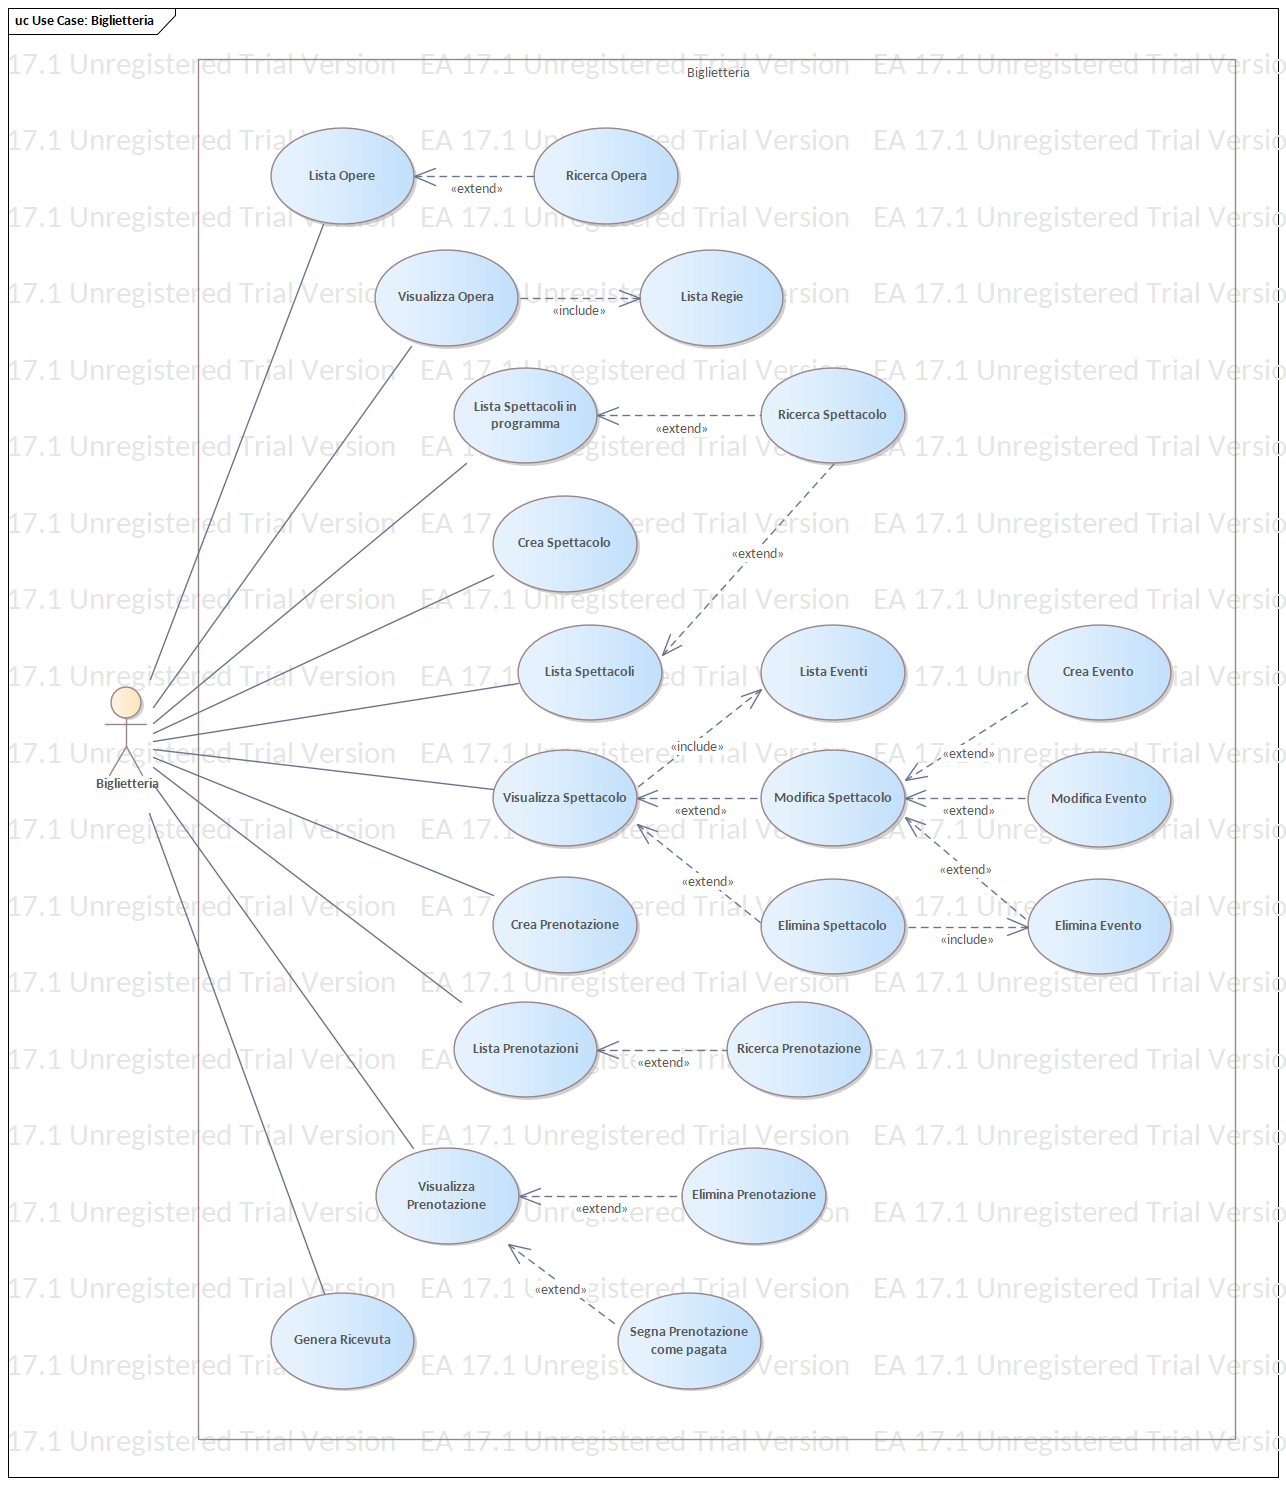
\includegraphics[scale=0.6]{imgs/use_case/biglietteria}
			\newpage
			
			\textbf{Descrizioni}
			% UC: Crea Spettacolo			[X]
% UC ext: Modifica Spettacolo		[X]
% UC ext: Elimina Spettacolo		[X]
% UC ext: Crea Evento			[X]
% UC ext: Modifica Evento		[X]
% UC ext: Elimina Evento		[X]
% UC: Lista Prenotazioni		[X]
% UC ext: Ricerca Prenotazione		[X]
% UC ext: Elimina Prenotazione	[X]
% UC ext: Segna Prenotazione come pagata	[X]

\renewcommand{\attori}{Biglietteria \\ Amministratore}
% ID: 14-23


{\ucTable	% UC: Crea Spettacolo
{	% Caso d'uso
	Crea Spettacolo
	
}{	% ID
	\increaseCount{classId}
	
}{	% Breve descrizione
	L'Utente crea uno Spettacolo da svolgere nel teatro.
	
}{	% Attori Primari
	\attori
	
}{	% Precondizioni
	\begin{enumerate}
        \item L'Utente si trova nella sezione SPETTACOLI.
        % "si trova"(5)
        % "SPETTACOLI"(8)
    \end{enumerate}
	
}{	% Sequenza Eventi Principale
	\begin{enumerate}
        \item L'Utente avvia il caso d'uso selezionando il comando "Crea Spettacolo".
        \item Il sistema mostra una interfaccia per inserire dati e impostazioni dello Spettacolo.
        \item L'Utente inserisce le informazioni dello Spettacolo.
        \item L'Utente conferma la creazione.
        \item Il sistema verifica i dati e li salva in memoria.
    \end{enumerate}
	
}{	% Postcondizioni
	\begin{enumerate}
        \item L'Utente crea uno Spettacolo.
    \end{enumerate}
	
}{	% Sequenza Eventi Alternativa
} }

{\ucExtTable	% UC EXT: Modifica Spettacolo
{	% Caso d'uso
	Modifica Spettacolo
	
}{	% ID
	\increaseCount{classId}
	
}{	% Breve descrizione
	L'Utente modifica le informazioni di uno Spettacolo.
	
}{	% Attori Primari
	\attori
	
}{	% Precondizioni
	\begin{enumerate}
        \item L'Utente si trova nella sezione SPETTACOLI.
        % "si trova"(5)
    \end{enumerate}
	
}{	% Sequenza Eventi Principale
	\begin{enumerate}
        \item L'Utente avvia il caso d'uso selezionando il comando "Modifica" associato ad uno Spettacolo.
        \item Il sistema consente all'Utente di modificare le informazioni dell'Opera.
        \item L'Utente inserisce le modifiche desiderate e le conferma.
        \item Il sistema verifica i dati e li salva in memoria.
    \end{enumerate}
	
}{	% Postcondizioni
	\begin{enumerate}
        \item L'Utente effettua la modifica di uno Spettacolo.
    \end{enumerate}
	
} }

{\ucExtTable	% UC EXT: Elimina Spettacolo
{	% Caso d'uso
	Elimina Spettacolo
	
}{	% ID
	\increaseCount{classId}
	
}{	% Breve descrizione
	L'Utente elimina uno Spettacolo dalla lista di Spettacoli memorizzati.
	
}{	% Attori Primari
	\attori
	
}{	% Precondizioni
	\begin{enumerate}
        \item L'Utente si trova nella sezione SPETTACOLI.
        % "si trova"(5)
    \end{enumerate}
	
}{	% Sequenza Eventi Principale
	\begin{enumerate}
        \item L'Utente avvia il caso d'uso selezionando il comando "Elimina" associato ad uno Spettacolo.
        \item Il sistema richiede all'Utente di confermare l'intenzione di eliminare lo Spettacolo.
        \item L'Utente conferma l'elimina.
        \item Il sistema verifica che non ci siano Eventi associati allo Spettacolo e lo elimina permanentemente.
        % "e la elimina permanentemente"(10)
    \end{enumerate}
	
}{	% Postcondizioni
	\begin{enumerate}
        \item L'Utente effettua l'eliminazione di uno Spettacolo.
    \end{enumerate}
	
} }

{\ucExtTable	% UC EXT: Crea Evento
{	% Caso d'uso
	Crea Evento
	
}{	% ID
	\increaseCount{classId}
	
}{	% Breve descrizione
	L'Utente crea un'Evento per uno Spettacolo.
	
}{	% Attori Primari
	\attori
	
}{	% Precondizioni
	\begin{enumerate}
        \item L'Utente sta visualizzando uno Spettacolo.
    \end{enumerate}
	
}{	% Sequenza Eventi Principale
	\begin{enumerate}
        \item L'Utente avvia il caso d'uso selezionando il comando "Crea Evento".
        \item Il sistema mostra una interfaccia per inserire la data e ora dell'Evento.
        \item L'Utente inserisce le informazioni dell'Evento.
        \item L'Utente conferma la creazione.
        \item Il sistema verifica i dati e li salva in memoria.
    \end{enumerate}
	
}{	% Postcondizioni
	\begin{enumerate}
        \item Il nuovo Evento è memorizzato e immediatamente visibile a tutti gli utenti.
    \end{enumerate}
	
} }

{\ucExtTable	% UC EXT: Modifica Evento
{	% Caso d'uso
	Modifica Evento
	
}{	% ID
	\increaseCount{classId}
	
}{	% Breve descrizione
	L'Utente modifica le informazioni di un'Evento.
	
}{	% Attori Primari
	\attori
	
}{	% Precondizioni
	\begin{enumerate}
        \item L'Utente sta visualizzando un'Opera.
    \end{enumerate}
	
}{	% Sequenza Eventi Principale
	\begin{enumerate}
        \item L'Utente avvia il caso d'uso selezionando il comando "Modifica" associato ad un'Evento.
        \item Il sistema consente all'Utente di modificare la data e ora dell'Evento.
        \item L'Utente inserisce le modifiche desiderate e le conferma.
        \item Il sistema verifica i dati e li salva in memoria.
    \end{enumerate}
	
}{	% Postcondizioni
	\begin{enumerate}
        \item Le modifiche apportate sono memorizzate e immediatamente disponibili a tutti gli utenti.
    \end{enumerate}
	
} }

{\ucExtTable	% UC EXT: Elimina Evento
{	% Caso d'uso
	Elimina Evento
	
}{	% ID
	\increaseCount{classId}
	
}{	% Breve descrizione
	L'Utente elimina un'Evento dalla lista di Eventi associati allo Spettacolo.
	
}{	% Attori Primari
	\attori
	
}{	% Precondizioni
	\begin{enumerate}
        \item L'Utente sta visualizzando un'Opera.
    \end{enumerate}
	
}{	% Sequenza Eventi Principale
	\begin{enumerate}
        \item L'Utente avvia il caso d'uso selezionando il comando "Elimina" associato ad un'Evento.
        \item Il sistema richiede all'Utente di confermare l'intenzione di eliminare l'Evento.
        \item L'Utente conferma l'elimina.
        \item Il sistema verifica che non ci siano Prenotazioni associate all'Evento e lo elimina permanentemente.
        % "e la elimina permanentemente"(10)
    \end{enumerate}
	
}{	% Postcondizioni
	\begin{enumerate}
        \item L'Utente effettua l'eliminazione di un'Evento.
    \end{enumerate}
	
} }

{\ucTable	% UC: Lista Prenotazioni
{	% Caso d'uso
	Lista Prenotazioni
	
}{	% ID
	\increaseCount{classId}
	
}{	% Breve descrizione
	L'Utente visualizza l'elenco delle Prenotazione memorizzate.
    % "visualizza"
	
}{	% Attori Primari
	\attori
	
}{	% Precondizioni
	\begin{enumerate}
        \item L'Utente si trova nella sezione PRENOTAZIONI.
    \end{enumerate}
	
}{	% Sequenza Eventi Principale
	\begin{enumerate}
        \item Il sistema mostra a schermo il nominativo e l'ora di emmisione di tutte Prenotazioni memorizzate.
        % "mostra a schermo <oggetto>"(3)
        \item Il sistema permette all'Utente di visualizzare in più dettaglio ed eliminare le Prenotazioni.
        % "visualizza in più dettaglio"(9)
        \item[] \textbf{punto di estensione:} Ricerca Prenotazione
    \end{enumerate}
	
}{	% Postcondizioni
	\begin{enumerate}
        \item La lista di Prenotazioni memorizzate viene visualizzata a schermo.
        % "visualizza a schermo <oggetto>"(4)
    \end{enumerate}
	
}{	% Sequenza Eventi Alternativa
} }


{\ucExtTable	% UC EXT: Elimina Prenotazione
{	% Caso d'uso
    Elimina Prenotazione
    
}{	% ID
    \increaseCount{classId}
    
}{	% Breve descrizione
    L'Utente elimina una Sezione dalla lista di Sezioni memorizzate.
    
}{	% Attori Primari
    \attori
}{	% Precondizioni
    \begin{enumerate}
        \item L'Utente si trova nella sezione PRENOTAZIONI.
    \end{enumerate}
    
}{	% Sequenza Eventi Principale
    \begin{enumerate}
        \item L'Utente avvia il caso d'uso selezionando il comando "Elimina" associato ad una Prenotazione.
        \item Il sistema richiede all'Utente di confermare l'intenzione di eliminare la Prenotazione.
        \item L'Utente conferma l'elimina.
        \item Il sistema elimina la Prenotazione permanentemente.
        % "e la elimina permanentemente"(10)
    \end{enumerate}
    
}{	% Postcondizioni
    \begin{enumerate}
        \item L'Utente effettua l'eliminazione di una Prenotazione.
    \end{enumerate}
		
} }


{\ucExtTable	% UC EXT: Ricerca Prenotazione
{	% Caso d'uso
	Ricerca Prenotazione
	
}{	% ID
	\increaseCount{classId}
	
}{	% Breve descrizione
	L'Utente filtra la lista delle Prenotazioni una parola chiave ricercata nel nominativo.
	
}{	% Attori Primari
	\attori
	
}{	% Precondizioni
	\begin{enumerate}
        \item L'Utente si trova nella sezione PRENOTAZIONI.
			% "si trova"(5)
    \end{enumerate}
	
}{	% Sequenza Eventi Principale
	\begin{enumerate}
        \item L'Utente effettua una ricerca specificando una chiave di ricerca.
        \item Le Prenotazioni che non contengono la parola chiave nel suo nominativo non vengono incluse nella lista risultante.
        % "nel suo nominativo"
        % "non vengono inclusi"
    \end{enumerate}
	
}{	% Postcondizioni
	\begin{enumerate}
        \item La lista risultante è filtrata. % Versión precedente: L'Utente visualizza l'elenco filtrato.
    \end{enumerate}
	
} }

{\ucExtTable	% UC EXT: Segna Prenotazione come Pagata
{	% Caso d'uso
	Segna Prenotazione come Pagata
	
}{	% ID
	\increaseCount{classId}
	
}{	% Breve descrizione
	L'Utente segna una Prenotazione come \emph{pagata}.
	
}{	% Attori Primari
	\attori
	
}{	% Precondizioni
	\begin{enumerate}
        \item L'Utente sta visualizzando una Prenotazione.
    \end{enumerate}
	
}{	% Sequenza Eventi Principale
	\begin{enumerate}
        \item L'Utente avvia il caso d'uso selezionando il comando "Segna come \emph{pagata}" associato ad una Prenotazione.
        \item Il sistema chiede conferma all'Utente. % - Nella prattica, non chiede mai conferma
        \item L'Utente conferma l'assegnamento della Prenotazione come \emph{pagata}.
        \item Il sistema effettua l'assegnamento.
    \end{enumerate}
	
}{	% Postcondizioni
	\begin{enumerate}
        \item La Prenotazione è segnata come \emph{pagata}.
    \end{enumerate}
	
} }
			\newpage
			
		\subsubsection{Amministratore}
			\textbf{Diagramma} \\ \\ 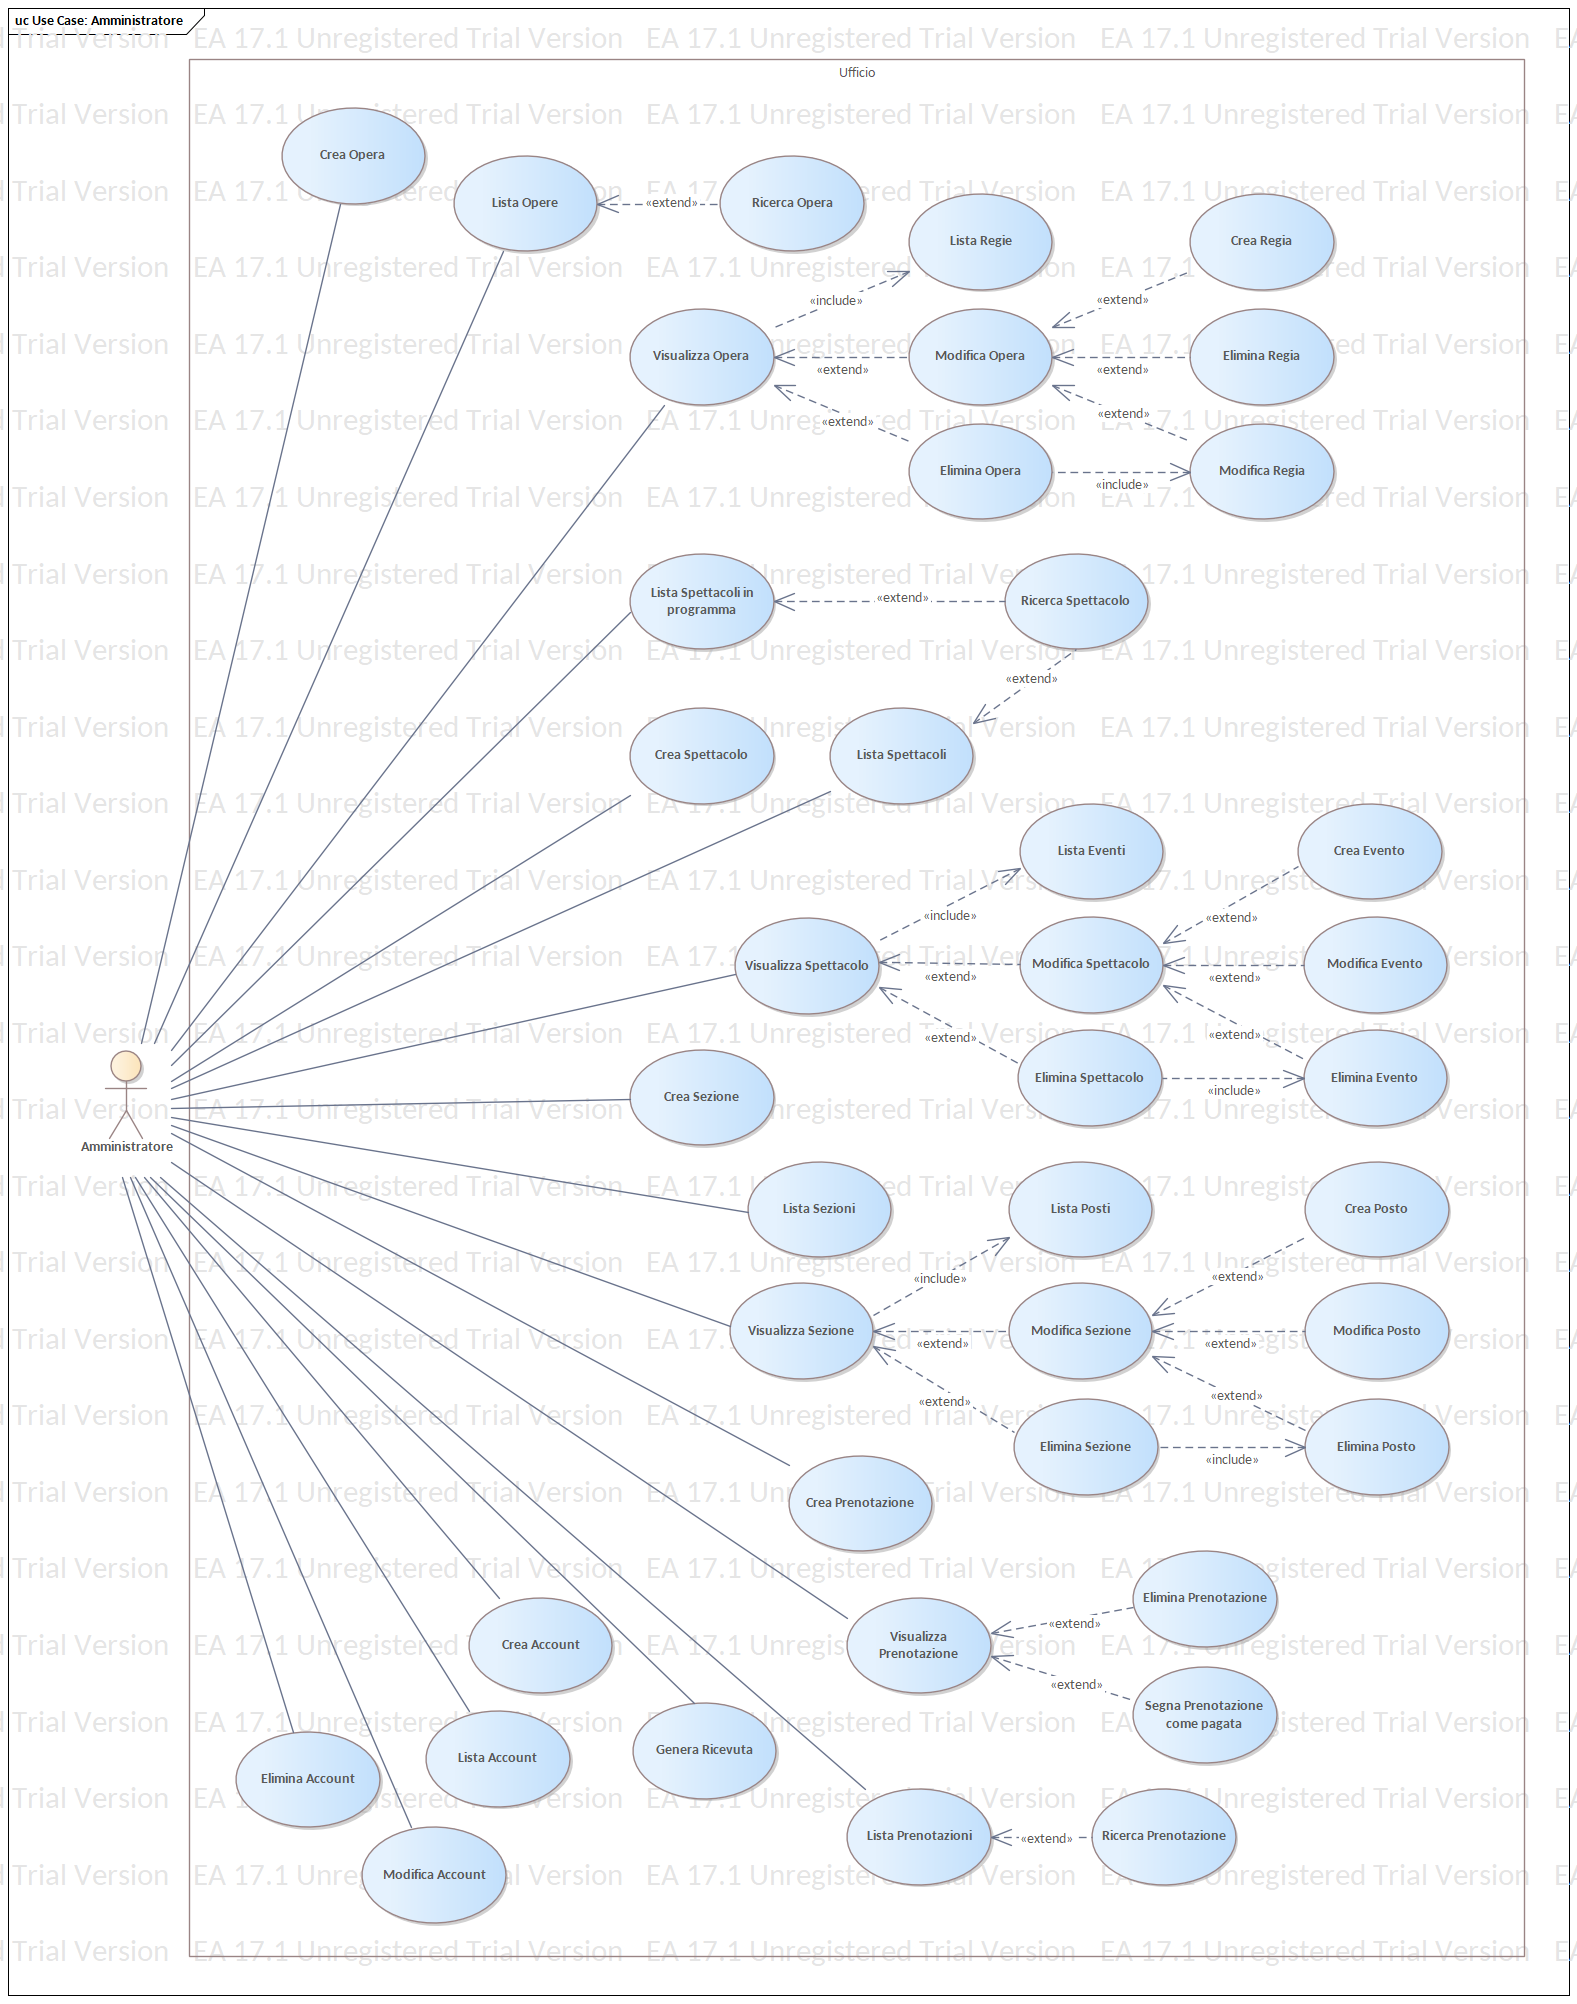
\includegraphics[scale=0.55]{imgs/use_case/amministratore}
			\newpage
			
			\textbf{Descrizioni}
			% "e la elimina permanentemente"(10): Usato nei passi del mainflow nei casi d'uso di elimina
%   dove si indica l'eliminazione.


% UC: Crea Opera		[X]
% UC ext: Modifica Opera	[X]
% UC ext: Elimina Opera	[X]
% UC ext: Crea Regia		[X]
% UC ext: Modifica Regia	[X]
% UC ext: Elimina Regia	[X]
% UC: Crea Sezione		[X]
% UC: Lista Sezioni		[X]
% UC: Visualizza Sezione	[X]
% UC: Lista Posti		[X]
% UC ext: Modifica Sezione	[X]
% UC ext: Elimina Sezione	[X]
% UC: Crea Posto		[X]
% UC: Modifica Posto		[X]
% UC: Elimina Posto		[X]
% UC: Crea Account  [X]
% UC: Lista Account [X]
% UC: Modifica Account [X]
% UC: Elimina Account [X]

\renewcommand{\attori}{Amministratore}
% ID: 23-42

{\ucTable	% UC: Crea Opera
{	% Caso d'uso
	Crea Opera
	
}{	% ID
	\increaseCount{classId}
	
}{	% Breve descrizione
	L'Utente crea un'Opera da svolgere nel teatro.
	
}{	% Attori Primari
	\attori
	
}{	% Precondizioni
	\begin{enumerate}
        \item L'Utente si trova nella sezione INFORMAZIONI.
        % "INFORMAZIONI"(2)
    \end{enumerate}
	
}{	% Sequenza Eventi Principale
	\begin{enumerate}
        \item L'Utente avvia il caso d'uso selezionando il comando "Crea Opera".
        \item Il sistema mostra una interfaccia per inserire dati e impostazioni dell'Opera.
        \item L'Utente inserisce le informazioni dell'Opera.
        \item L'Utente conferma la creazione.
        \item Il sistema verifica i dati e li salva in memoria.
    \end{enumerate}
	
}{	% Postcondizioni
	\begin{enumerate}
        \item La nuova Opera è memorizzata e immediatamente visibile a tutti gli Utenti.
    \end{enumerate}
	
}{	% Sequenza Eventi Alternativa
} }

{\ucExtTable	% UC EXT: Modifica Opera
{	% Caso d'uso
	Modifica Opera
	
}{	% ID
	\increaseCount{classId}
	
}{	% Breve descrizione
	L'Utente modifica le informazioni di un'Opera.
	
}{	% Attori Primari
	\attori
	
}{	% Precondizioni
	\begin{enumerate}
        \item L'Utente si trova nella sezione INFORMAZIONI.
        % "si trova"(5)
        % "INFORMAZIONI"(2)
    \end{enumerate}
	
}{	% Sequenza Eventi Principale
	\begin{enumerate}
        \item L'Utente avvia il caso d'uso selezionando il comando "Modifica" associato ad un'Opera.
        \item Il sistema consente all'Utente di modificare le informazioni dell'Opera.
        \item L'Utente inserisce le modifiche desiderate e le conferma.
        \item Il sistema verifica i dati e li salva in memoria.
    \end{enumerate}
	
}{	% Postcondizioni
	\begin{enumerate}
        \item Le modifiche apportate sono memorizzate e immediatamente disponibili a tutti gli Utenti.
    \end{enumerate}
	
} }

{\ucExtTable	% UC EXT: Elimina Opera
{	% Caso d'uso
	Elimina Opera
	
}{	% ID
	\increaseCount{classId}
	
}{	% Breve descrizione
	L'Utente elimina un'Opera dalla lista di Opere memorizzate.
	
}{	% Attori Primari
	\attori
	
}{	% Precondizioni
	\begin{enumerate}
        \item L'Utente si trova nella sezione INFORMAZIONI.
        % "si trova"(5)
    \end{enumerate}
	
}{	% Sequenza Eventi Principale
	\begin{enumerate}
        \item L'Utente avvia il caso d'uso selezionando il comando "Elimina" associato ad un'Opera.
        \item Il sistema richiede all'Utente di confermare l'intenzione di eliminare l'Opera.
        \item L'Utente conferma l'elimina.
        \item Il sistema verifica che non ci siano Regie associate all'Opera e la elimina permanentemente.
        % "e la elimina permanentemente"(10)
    \end{enumerate}
	
}{	% Postcondizioni
	\begin{enumerate}
        \item L'Utente effettua l'eliminazione di un'Opera.
    \end{enumerate}
	
} }

{\ucExtTable	% UC EXT: Crea Regia
{	% Caso d'uso
	Crea Regia
	
}{	% ID
	\increaseCount{classId}
	
}{	% Breve descrizione
	L'Utente crea una nuova Regia per un'Opera.
	
}{	% Attori Primari
	\attori
	
}{	% Precondizioni
    \begin{enumerate}
        \item L'Utente sta visualizzando un'Opera.
    \end{enumerate}
	
}{	% Sequenza Eventi Principale
    \begin{enumerate}
        \item L'Utente avvia il caso d'uso selezionando il comando "Crea Regia".
        \item Il sistema mostra una interfaccia per inserire dati e impostazioni della Regia.
        \item L'Utente inserisce le informazioni della Regia.
        \item L'Utente conferma la creazione.
        \item Il sistema verifica i dati e li salva in memoria.
    \end{enumerate}
	
}{	% Postcondizioni
	\begin{enumerate}
        \item La nuova Regia è memorizzata e immediatamente visibile a tutti gli Utenti.
    \end{enumerate}
	
} }

{\ucExtTable	% UC EXT: Modifica Regia
{	% Caso d'uso
	Modifica Regia
	
}{	% ID
	\increaseCount{classId}
	
}{	% Breve descrizione
	L'Utente modifica le informazioni di una Regia.
	
}{	% Attori Primari
	\attori
	
}{	% Precondizioni
	\begin{enumerate}
        \item L'Utente sta visualizzando un'Opera.
    \end{enumerate}
	
}{	% Sequenza Eventi Principale
    \begin{enumerate}
        \item L'Utente avvia il caso d'uso selezionando il comando "Modifica" associato ad una Regia.
        \item Il sistema consente all'Utente di modificare le informazioni della Regia.
        \item L'Utente inserisce le modifiche desiderate e le conferma.
        \item Il sistema verifica i dati e li salva in memoria.
    \end{enumerate}
	
}{	% Postcondizioni
	\begin{enumerate}
        \item Le modifiche apportate sono memorizzate e immediatamente disponibili a tutti gli Utenti.
    \end{enumerate}
	
} }

{\ucExtTable	% UC EXT: Elimina Regia
{	% Caso d'uso
	Elimina Regia
	
}{	% ID
	\increaseCount{classId}
	
}{	% Breve descrizione
	L'Utente elimina una Regia dalla lista di Regie associate all'Opera.
	
}{	% Attori Primari
	\attori
	
}{	% Precondizioni
	\begin{enumerate}
        \item L'Utente sta visualizzando un'Opera.
    \end{enumerate}
	
}{	% Sequenza Eventi Principale
    \begin{enumerate}
        \item L'Utente avvia il caso d'uso selezionando il comando "Elimina" associato ad una Regia.
        \item Il sistema richiede all'Utente di confermare l'intenzione di eliminare la Regia.
        \item L'Utente conferma l'elimina.
        \item Il sistema verifica che non ci siano Eventi associate alla Regia e la elimina permanentemente.
        % "e la elimina permanentemente"(10)
    \end{enumerate}
	
}{	% Postcondizioni
	\begin{enumerate}
        \item L'Utente effettua l'eliminazione di una Regia.
    \end{enumerate}
	
} }

{\ucTable	% UC: Crea Sezione
{	% Caso d'uso
	Crea Sezione
	
}{	% ID
	\increaseCount{classId}
	
}{	% Breve descrizione
	L'Utente crea una Sezione di Posti nel teatro.
	
}{	% Attori Primari
	\attori
	
}{	% Precondizioni
	\begin{enumerate}
        \item L'Utente si trova nella sezione TEATRO.
    \end{enumerate}
	
}{	% Sequenza Eventi Principale
	\begin{enumerate}
        \item L'Utente avvia il caso d'uso selezionando il comando "Crea Sezione".
        \item Il sistema mostra una interfaccia per inserire i dati della Sezione.
        \item L'Utente inserisce le informazioni della Sezione.
        \item L'Utente conferma la creazione.
        \item Il sistema verifica i dati e li salva in memoria.
    \end{enumerate}
	
}{	% Postcondizioni
	\begin{enumerate}
        \item L'Utente crea una Sezione.
        % \item La nuova Sezione è stata aggiunta alla Lista delle Sezioni.
    \end{enumerate}
	
}{	% Sequenza Eventi Alternativa
} }


{\ucTable	% UC: Lista Sezioni
	{	% Caso d'uso
		Lista Sezioni
		
	}{	% ID
		\increaseCount{classId}
		
	}{	% Breve descrizione
		L'Utente visualizza l'elenco delle Sezioni memorizzate.
        % "visualizza"
		
	}{	% Attori Primari
		\attori
	}{	% Precondizioni
		\begin{enumerate}
			\item L'Utente si trova nella sezione TEATRO.
		\end{enumerate}
		
	}{	% Sequenza Eventi Principale
		\begin{enumerate}
            \item Il sistema mostra a schermo tutte le Sezioni memorizzate.
            % "mostra a schermo <oggetto>"(3)
            \item Il sistema permette all'Utente di visualizzare in più dettaglio, modificare ed eliminare le Sezioni.
            % "visualizza in più dettaglio"(9)	
		\end{enumerate}
		
	}{	% Postcondizioni
		\begin{enumerate}
			\item La lista di Sezioni memorizzate viene visualizzata a schermo.
            % "visualizza a schermo <oggetto>"(4)
		\end{enumerate}
		
	}{	% Sequenza Eventi Alternativa
} }


{\ucTable	% UC: Visualizza Sezione
{	% Caso d'uso
    Visualizza Sezione
    
}{	% ID
    \increaseCount{classId}
    
}{	% Breve descrizione
    L'Utente visualizza le informazioni riguardo una singola Sezione.
    
}{	% Attori Primari
    \attori
}{	% Precondizioni
    \begin{enumerate}
        \item L'Utente si trova nella sezione TEATRO.
        % "si trova"(5)
    \end{enumerate}
    
}{	% Sequenza Eventi Principale
    \begin{enumerate}
        \item L'Utente richiede le informazioni di una Sezione.
        \item Il sistema mostra a schermo le informazioni.
        % "mostra a schermo <oggetto>"(3)
        \item \textbf{include}(Lista Posto) % - Non è corretto secondo l'altra usecase description
        \item[] \textbf{punto di estensione:} Crea Posto
    \end{enumerate}
    
}{	% Postcondizioni
    \begin{enumerate}
        \item Le informazioni della Sezione vengono visualizzate a schermo.
        % "visualizza a schermo <oggetto>"(4)
    \end{enumerate}
    
}{	% Sequenza Eventi Alternativa
} }


{\ucTable	% UC: Lista Posti
	{	% Caso d'uso
		Lista Posti
		
	}{	% ID
		\increaseCount{classId}
		
	}{	% Breve descrizione
		L'Utente visualizza la lista di Posti associati alla Sezione che sta visualizzando.
		
	}{	% Attori Primari
		\attori
	}{	% Precondizioni
		\begin{enumerate}
			\item L'Utente sta visualizzando una singola Sezione.
		\end{enumerate}
		
	}{	% Sequenza Eventi Principale
		\begin{enumerate}
            \item Il sistema mostra a schermo le informazioni essenziali di tutti i Posti associati alla Sezione.
            % "mostra a schermo <oggetto>"(3)
            % "associate"(6)
            \item Il sistema permette all'Utente di creare, modificare ed eliminare i Posti.		
		\end{enumerate}
		
	}{	% Postcondizioni
		\begin{enumerate}
			\item La lista di Posti associati alla Sezione viene visualizzata a schermo.
            % "visualizza a schermo <oggetto>"(4)
            % "associate"(6)
		\end{enumerate}
		
	}{	% Sequenza Eventi Alternativa
} }


{\ucExtTable	% UC EXT: Modifica Sezione
{	% Caso d'uso
	Modifica Sezione
	
}{	% ID
	\increaseCount{classId}
	
}{	% Breve descrizione
	L'Utente modifica le informazioni di una Sezione.
	
}{	% Attori Primari
	\attori
	
}{	% Precondizioni
	\begin{enumerate}
        \item L'Utente si trova nella sezione TEATRO.
        % "si trova"(5)
    \end{enumerate}
	
}{	% Sequenza Eventi Principale
	\begin{enumerate}
        \item L'Utente avvia il caso d'uso selezionando il comando "Modifica" associato ad una Sezione.
        \item Il sistema consente all'Utente di modificare le informazioni della Sezione, e.g. nome, descrizione.
        \item L'Utente inserisce le modifiche desiderate e le conferma.
        \item Il sistema verifica i dati e li salva in memoria.
    \end{enumerate}
	
}{	% Postcondizioni
	\begin{enumerate}
        \item L'Utente effettua la modifica di una Sezione.
    \end{enumerate}
	
} }

{\ucExtTable	% UC EXT: Elimina Sezione
{	% Caso d'uso
	Elimina Sezione
	
}{	% ID
	\increaseCount{classId}
	
}{	% Breve descrizione
	L'Utente elimina una Sezione dalla lista di Sezioni memorizzate.
	
}{	% Attori Primari
	\attori
	
}{	% Precondizioni
	\begin{enumerate}
        \item L'Utente si trova nella sezione TEATRO.
    \end{enumerate}
	
}{	% Sequenza Eventi Principale
	\begin{enumerate}
        \item L'Utente avvia il caso d'uso selezionando il comando "Elimina" associato ad una Sezione.
        \item Il sistema richiede all'Utente di confermare l'intenzione di eliminare la Sezione.
        \item L'Utente conferma l'elimina.
        \item Il sistema verifica che non ci siano Posti associati alla Sezione e la elimina permanentemente.
        % "e la elimina permanentemente"(10)
    \end{enumerate}
	
}{	% Postcondizioni
	\begin{enumerate}
        \item L'Utente effettua l'eliminazione di una Sezione.
    \end{enumerate}
	
} }

{\ucTable	% UC: Crea Posto
{	% Caso d'uso
	Crea Posto
	
}{	% ID
	\increaseCount{classId}
	
}{	% Breve descrizione
	L'Utente crea un Posto (o Posti) per una Sezione.
	
}{	% Attori Primari
	\attori
	
}{	% Precondizioni
	\begin{enumerate}
        \item L'Utente sta visualizzando una Sezione.
    \end{enumerate}
	
}{	% Sequenza Eventi Principale
	\begin{enumerate}
        \item L'Utente avvia il caso d'uso inserendo i dati necessario (fila e numero) nella pagina.
        \item \textbf{If} l'Utente sceglie di creare multipli Posti
            \begin{enumerate}
                \item Il sistema permette all'Utente di inserire un rango di numeri (per i Posti) nella pagina.
            \end{enumerate}
        \item L'Utente conferma la creazione.
        \item \textbf{For} ogni numero inserito nel campo di numeri % - Studiare/Corriggere
            \begin{enumerate}
                \item Il sistema verifica i dati e li salva in memoria.
            \end{enumerate}
    \end{enumerate}
	
}{	% Postcondizioni
	\begin{enumerate}
        \item Il nuovo Posto (o Posti) è memorizzato e immediatamente visibile a tutti gli Utenti.
    \end{enumerate}
	
}{	% Sequenza Eventi Alternativa
} }

{\ucTable	% UC: Modifica Posto
{	% Caso d'uso
	Modifica Posto
	
}{	% ID
	\increaseCount{classId}
	
}{	% Breve descrizione
	L'Utente modifica le informazioni di un Posto.
	
}{	% Attori Primari
	\attori
	
}{	% Precondizioni
	\begin{enumerate}
        \item L'Utente sta visualizzando una Sezione.
    \end{enumerate}
	
}{	% Sequenza Eventi Principale
	\begin{enumerate}
        \item L'Utente avvia il caso d'uso selezionando il comando "Modifica" associato ad un Posto.
        \item Il sistema consente all'Utente di modificare la fila e numero del Posto.
        \item L'Utente inserisce le modifiche desiderate e le conferma.
        \item Il sistema verifica i dati e li salva in memoria.
    \end{enumerate}
	
}{	% Postcondizioni
	\begin{enumerate}
        \item Le modifiche apportate sono memorizzate e immediatamente disponibili a tutti gli Utenti.
    \end{enumerate}
	
}{	% Sequenza Eventi Alternativa
} }

{\ucTable	% UC: Elimina Posto
{	% Caso d'uso
	Elimina Posto
	
}{	% ID
	\increaseCount{classId}
	
}{	% Breve descrizione
	L'Utente elimina un Posto dalla lista di Posti associati alla Sezione.
	
}{	% Attori Primari
	\attori
	
}{	% Precondizioni
	\begin{enumerate}
        \item L'Utente sta visualizzando una Sezione.
    \end{enumerate}
	
}{	% Sequenza Eventi Principale
	\begin{enumerate}
        \item L'Utente avvia il caso d'uso selezionando il comando "Elimina" associato ad un Posto.
        \item Il sistema verifica che non ci siano Prenotazioni associate al Posto e lo elimina permanentemente.
        % "e la elimina permanentemente"(10)
    \end{enumerate}
	
}{	% Postcondizioni
	\begin{enumerate}
        \item Le modifiche apportate sono memorizzate e immediatamente disponibili a tutti gli Utenti.
    \end{enumerate}
	
}{	% Sequenza Eventi Alternativa
} }


{\ucTable	% UC: Crea Account
{	% Caso d'uso
	Crea Account
	
}{	% ID
	\increaseCount{classId}
	
}{	% Breve descrizione
	L'Utente crea un Account di Biglietteria o Amministratore.
	
}{	% Attori Primari
	\attori
	
}{	% Precondizioni
	\begin{enumerate}
        \item L'Utente si trova nella sezione ACCOUNT.
    \end{enumerate}
	
}{	% Sequenza Eventi Principale
	\begin{enumerate}
        \item L'Utente avvia il caso d'uso selezionando il comando "Crea Account".
        \item Il sistema mostra una interfaccia per inserire username, password ed il ruolo dell'Account.
        \item L'Utente inserisce le informazioni dell'Account.
        \item L'Utente conferma la creazione.
        \item Il sistema verifica i dati e li salva in memoria.
    \end{enumerate}
	
}{	% Postcondizioni
	\begin{enumerate}
        \item Il nuovo Account è memorizzato e immediatamente accessibile. % - REVISARE
    \end{enumerate}
	
}{	% Sequenza Eventi Alternativa
} }


{\ucTable	% UC: Lista Account
	{	% Caso d'uso
		Lista Account
		
	}{	% ID
		\increaseCount{classId}
		
	}{	% Breve descrizione
		L'Utente visualizza la lista di Account memorizzati.
        % "visualizza"
        % "memorizzate"(1)
		
	}{	% Attori Primari
		\attori
		
	}{	% Precondizioni
		\begin{enumerate}
			\item L'Utente si trova nella sezione ACCOUNT.
			% "si trova"(5)
		\end{enumerate}
		
	}{	% Sequenza Eventi Principale
		\begin{enumerate}
			\item Il sistema mostra a schermo l'username di tutti gli Account memorizzati.
            % "mostra a schermo <oggetto>"(3)
            \item Il sistema permette all'Utente di modificare ed eliminare gli Account.
            % "visualizza in più dettaglio"(9)
		\end{enumerate}
		
	}{	% Postcondizioni
		\begin{enumerate}
			\item La lista di Account memorizzati viene visualizzata a schermo.
			% "visualizza a schermo <oggetto>"(4)
		\end{enumerate}
		
	}{	% Sequenza Eventi Alternativa
} }


{\ucExtTable	% UC EXT: Modifica Account
{	% Caso d'uso
	Modifica Account
	
}{	% ID
	\increaseCount{classId}
	
}{	% Breve descrizione
	L'Utente modifica le informazioni di un Account.
	
}{	% Attori Primari
	\attori
	
}{	% Precondizioni
	\begin{enumerate}
        \item L'Utente si trova nella sezione ACCOUNT.
        % "si trova"(5)
    \end{enumerate}
	
}{	% Sequenza Eventi Principale
	\begin{enumerate}
        \item L'Utente avvia il caso d'uso selezionando il comando "Modifica" associato ad un Account.
        \item Il sistema consente all'Utente di modificare la password ed il ruolo dell'Account.
        \item L'Utente inserisce le modifiche desiderate e le conferma.
        \item Il sistema verifica i dati e li salva in memoria.
    \end{enumerate}
	
}{	% Postcondizioni
	\begin{enumerate}
        \item Le modifiche apportate sono memorizzate e immediatamente disponibili a tutti gli Utenti.
    \end{enumerate}
	
} }


{\ucExtTable	% UC EXT: Elimina Account
{	% Caso d'uso
	Elimina Account
	
}{	% ID
	\increaseCount{classId}
	
}{	% Breve descrizione
	L'Utente elimina un Account dalla lista di Account memorizzate.
	
}{	% Attori Primari
	\attori
	
}{	% Precondizioni
	\begin{enumerate}
        \item L'Utente si trova nella sezione ACCOUNT.
        % "si trova"(5)
    \end{enumerate}
	
}{	% Sequenza Eventi Principale
	\begin{enumerate}
        \item L'Utente avvia il caso d'uso selezionando il comando "Elimina" associato ad un Account.
        \item Il sistema richiede all'Utente di confermare l'intenzione di eliminare l'Account.
        \item L'Utente conferma l'elimina.
        \item Il sistema elimina l'Account permanentemente.
        % "e la elimina permanentemente"(10)
    \end{enumerate}
	
}{	% Postcondizioni
	\begin{enumerate}
        \item L'Utente effettua l'eliminazione di un Account.
    \end{enumerate}
	
} }
	
	\subsection{Matrice di mapping}
	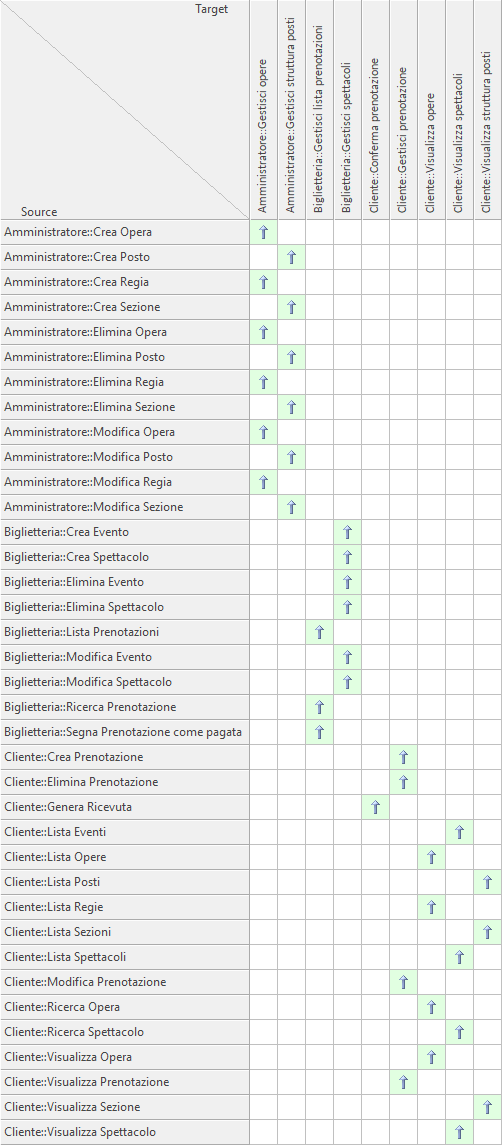
\includegraphics[height=\textheight]{imgs/matrice/matrice}
